\section {Capacitor Parameters}
This section will begin by describing some of the practical uses of capacitors and then transition into the various parameters that are used to describe capacitors. Section: \ref{sec:regression} will show a method which allows these parameters to be extrapolated from empirical data.

\subsection{Practical Capacitor Uses}

The most basic reason for wanting to use capacitors is that they  have the ability to store charge; the ability to store electrical energy. Capacitors have the ability to store and release electrical energy quickly, in order to be able to react to the needs of the circuit. This section will describe some of the most common uses for capacitors.

\subsubsection{Bypassing}
\begin{figure}[ht!]
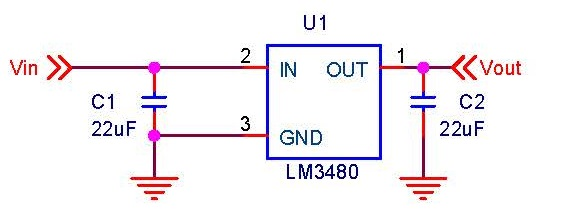
\includegraphics[keepaspectratio=true,scale=.5]{./figures/parameters/bypass.jpg}
\centering
\caption{Power Supply Bypassing Circuit}
\label{bypass}
\end{figure}


One of the most common uses of capacitors is in power supply bypassing. Capacitors are nearly always attached from a power rail to ground on a supply or IC. They provide a reservoir of charge that limits inductive voltage spikes, such as when a digital circuit switches, and limits voltage dips, caused by things such as a current surge when a processor boots.
Both LDOs (Figure: \ref{fig:bypass}) and switchers use bypass capacitors on their input and output voltage rails. Input capacitors are divided into two main categories, ripple reduction and bulk. Ripple reduction capacitors need a low \gls{esr} (Section: \ref{sec:ESR}) and are meant to decrease the magnitude of any AC signals that ride on top of the input DC voltage. Bulk capacitors are meant to deliver surge currents. Output capacitors have a similar purpose as input capacitors. The main difference is in the case of switching power supplies. In that application, the output capacitor is a major component in the feedback loop. It contributes to both the transient and stability properties of the switcher.

\subsubsection{Analog Filtering}
\begin{figure}
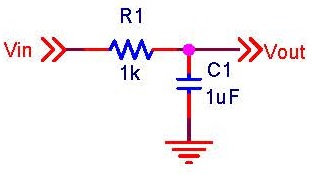
\includegraphics[keepaspectratio=true,scale=.5]{./figures/parameters/analogFiltering.jpg}
\centering
\caption{Analog Filtering Circuit}
%\cite{capSite_df_vs_temp}
\label{analogFiltering}
\end{figure}

Another use for capacitors is in analog filtering. The low-pass filter in Figure: \ref{fig:analogFiltering} attenuates frequencies above a cutoff point, set by the values of the resistor and capacitor. Low pass filters are needed in many applications, such as anti-aliasing, clock filtering, and integration.

\subsubsection{DC Blocking}
\begin{figure}[ht!]
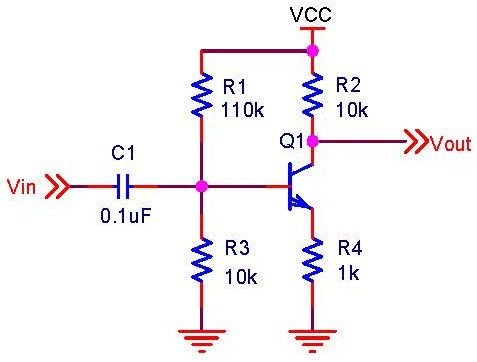
\includegraphics[keepaspectratio=true,scale=.5]{./figures/parameters/dcBlocking.jpg}
\centering
\caption{DC Blocking Capacitor}
\cite{hh}[ch 2.2.7 fig 2.35 pg 88]
\label{fig:dcBlock}
\end{figure}

Designers often take advantage of a capacitor's characteristic of passing AC current while blocking DC current. As in Figure: \ref{fig:dcBlock}, a capacitor can be used to block a DC offset before an amplifier.

\subsubsection{Oscillators}
\begin{figure}[ht!]
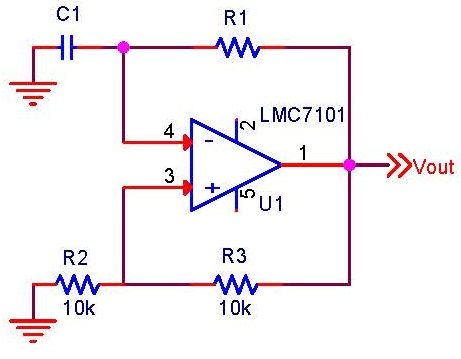
\includegraphics[keepaspectratio=true,scale=.5]{./figures/parameters/oscillator.jpg}
\centering
\caption{Oscillator Circuit}
\cite{hh}[ch 5.13 fig 5.29 pg 285]
\label{fig:oscillator}
\end{figure}


Stable capacitors of a very specific value are required to make a parallel resonant oscillator function properly (Figure: \ref{fig:oscillator}). These oscillators provide the clock base for most modern digital circuits using microcontroller.

\subsection{Capacitance}

There is a distinct difference between a capacitor and capacitance. While a capacitor's dominant characteristic is capacitance, it cannot be modeled entirely as such in most practical applications. There are also various inductive and resistive components to a capacitor that are important in various circumstances.

\begin{equation}
\label{equ:cqv}
C=\frac{Q}{V}
\end{equation}

Capacitance is the ability to store electrical charge. Equation: \eqref{equ:cqv} shows that capacitance is stored charge that is spread throughout a volume. A device that can store a lot of charge in a small space has a large capacitance. The basic equation for a commercial capacitor is seen in Equation: \eqref{equ:parPlateCap}.

\begin{equation}
\label{equ:parPlateCap}
C = \frac{\epsilon _0 A}{d}
\end{equation}

When using a capacitor in a single-pole low-pass filter, the cutoff frequency can be determined by Equation: \eqref{equ:lpfilter_eqn}. The circuit designer chooses a value for C and R in order to meet the cutoff frequency restraint.

\begin{equation}
\label{equ:lpfilter_eqn}
f = \frac{1}{2\pi RC}
\end{equation}

Varying the capacitance used in the filter moves the cutoff frequency and consequently produces a different response in the filter. The effect of this can be seen in Figure: \ref{fig:lpFiltVarC}.

\begin{figure}[ht!]
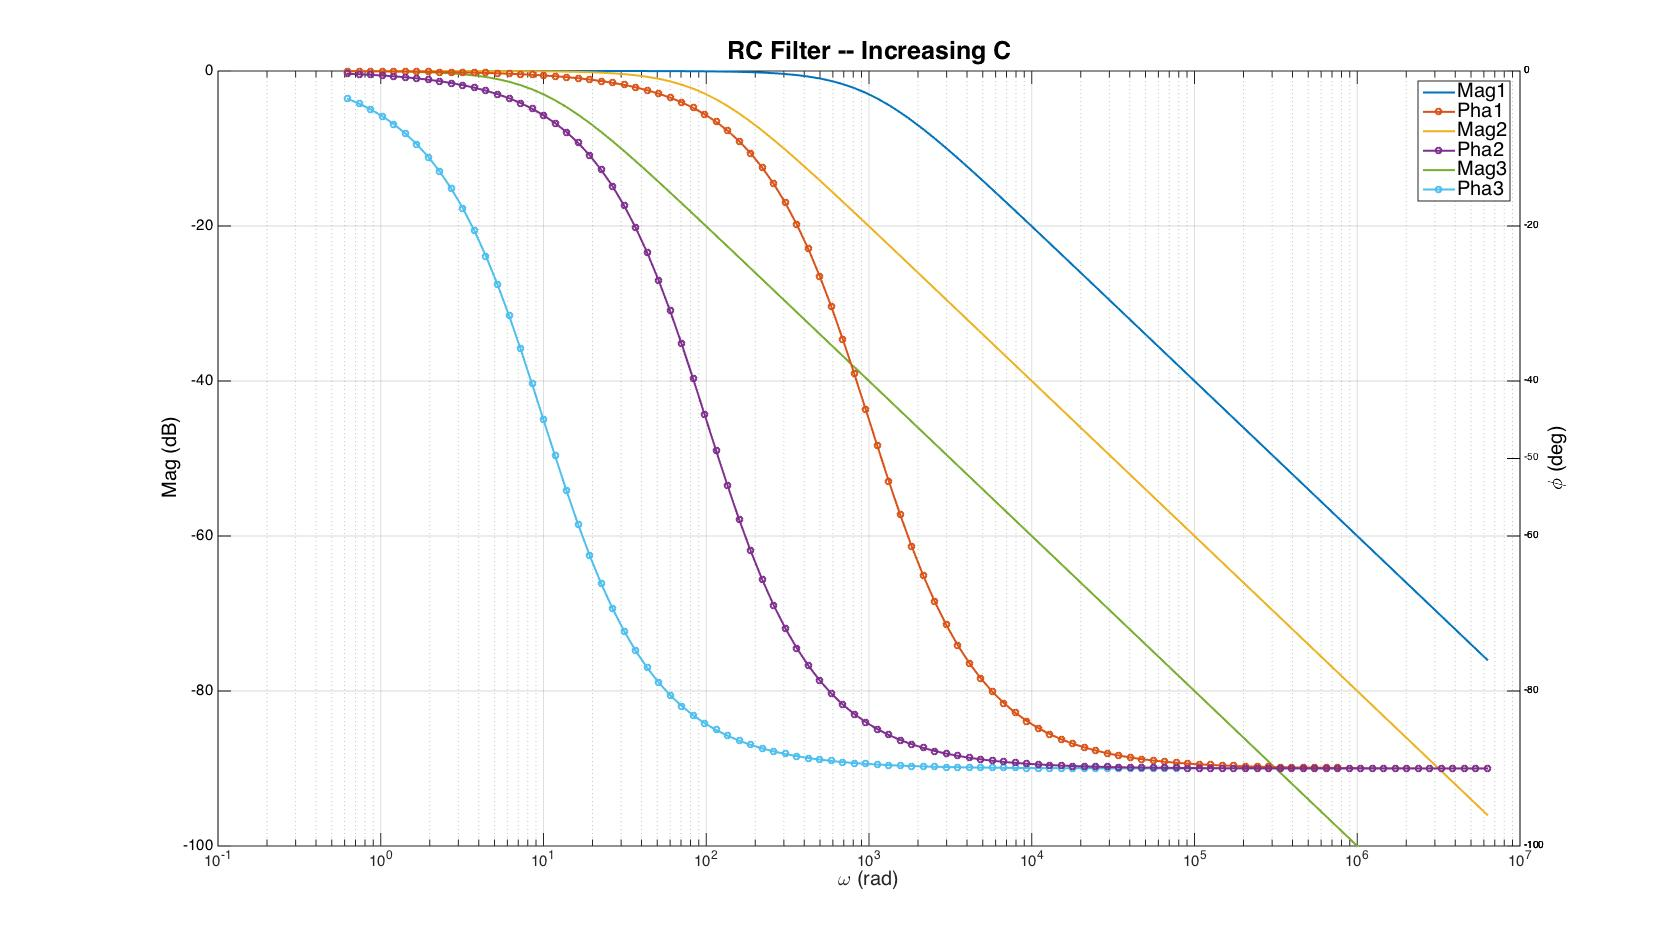
\includegraphics[keepaspectratio=true,width=6in]{./figures/parameters/lpFiltVarC.jpg}
\centering
\caption{Low Pass Filter -- Varying C}
\label{fig:lpFiltVarC}
\end{figure}


\subsection{Impedance}

The impedance of a capacitor is the ``AC resistance'' of the device. It determines the AC current that will flow when an AC voltage is applied to the capacitor via Ohm's law (Equation: \eqref{equ:capOhmsEqn}). Real capacitors have a complicated impedance equation, but ideal capacitors have a much simpler representation, as seen in Equation: \eqref{equ:capImpEqu}.

\begin{equation}
\label{equ:capOhmsEqn}
\vec{V} = \vec{I} \vec{Z}
\end{equation}

\begin{equation}
\label{equ:capImpEqu}
\vec{Z} = \frac{1}{j\omega C}
\end{equation}

\begin{equation}
\label{equ:capMagEqn}
Z = |\vec{Z}| = \frac{1}{\omega C}
\end{equation}

In most AC applications designers are interested in the magnitude of the impedance. Real capacitors have a more complicated impedance, but an ideal capacitor's magnitude equation can be simplified down to Equation \eqref{equ:capMagEqn}. When capacitors are used in bypassing power supplies, the goal is to have a low impedance for common or expected noise frequencies. Using a large valued capacitor to bypass a wide range of frequencies does not work in practical situations due to parasitics in a real capacitor. The parasitic elements, described in the following sections, cause various undesirable effects, such as the impedance of a capacitor increasing after a certain frequency. This results in a more complicated impedance plot than the ideal version shown in Figure: \ref{fig:cap}.

\begin{figure}
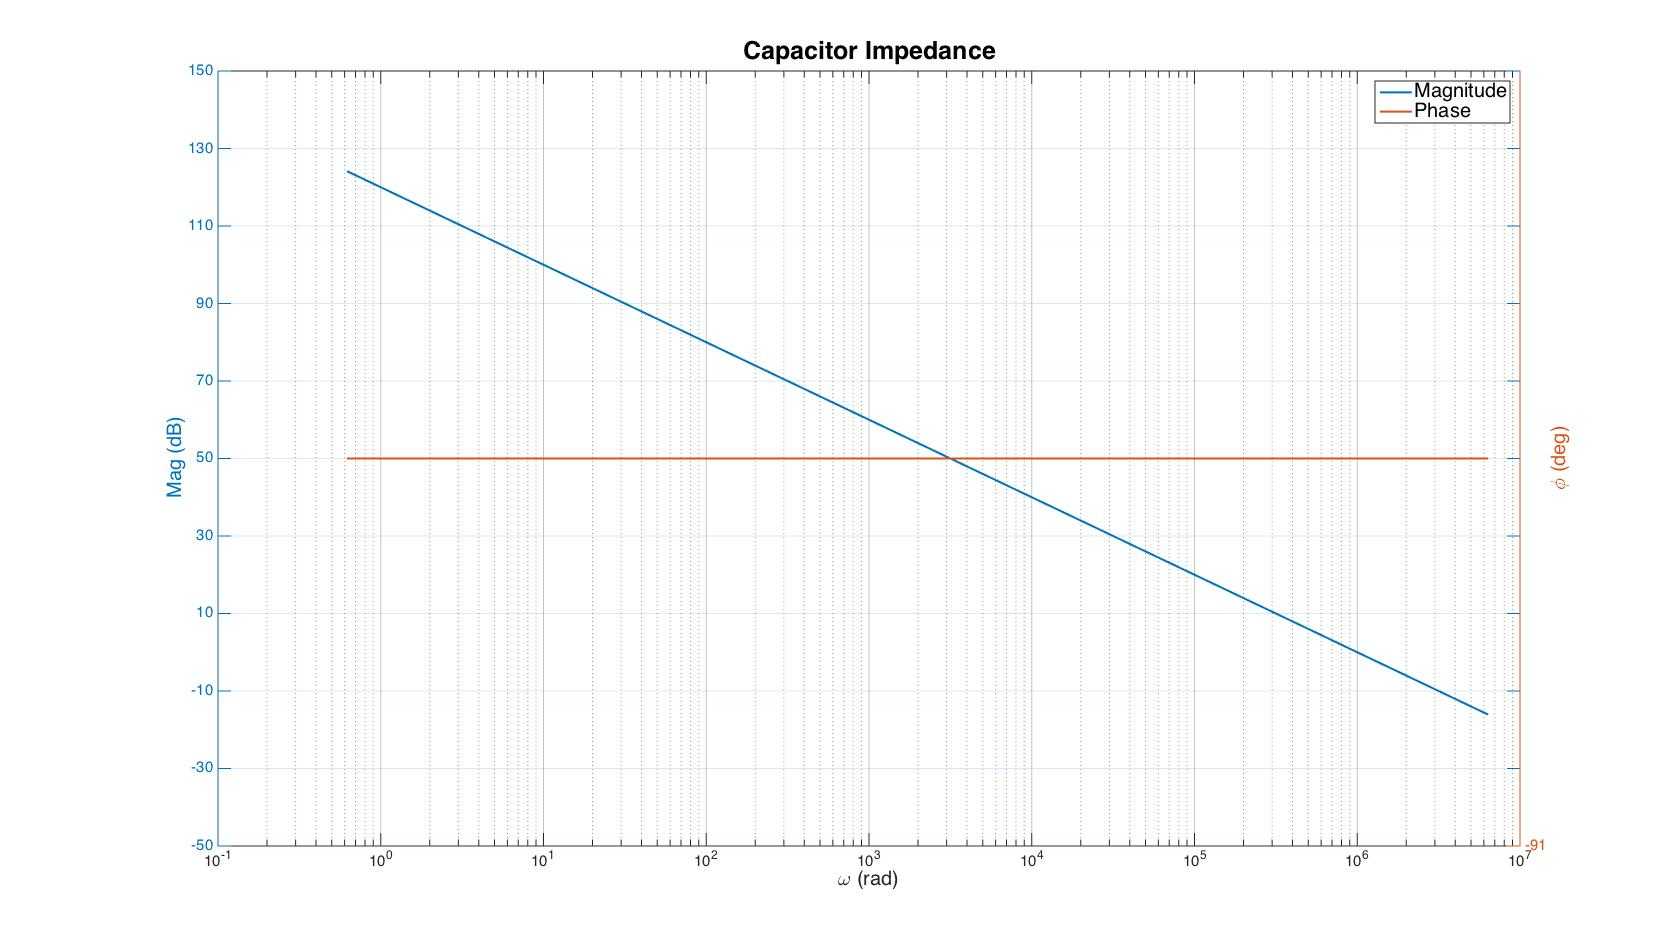
\includegraphics[keepaspectratio=true,width=6in]{./figures/parameters/cap.jpg}
\centering
\caption{Capacitor Magnitude Over Frequency}
\label{fig:cap}
\end{figure}


\subsection{Phase}

The phase of a combination of resistive and reactive components can be written as in Equation: \eqref{equ:capPhEqn}.

\begin{equation}
\label{equ:capPhEqn}
\phi = tan^{-1}[\frac{X_c}{R_c}]
\end{equation}

For an ideal capacitor, having no resistance and only capacitance, the phase angle can be simplified to:

\begin{equation}
\label{equ:capImpEqu2}
\phi = -i = -90^0
\end{equation}

The practical implication of this is seen in the phase response of a low pass filter (Figure: \ref{fig:lpFiltVarC}). The capacitor introduces a phase lag relative to the input signal's frequency. If you would compare the input and output signals in time, the output's peak would lag behind the input's by the phase amount predicted in the phase response.


\subsection{ESL}

The \gls{esl} of a capacitor is a lumped estimate of all of the inductive components of a capacitor. It is typically modeled as an inductor in series with the bulk capacitance (See Figure \ref{fig:eslModel}).

\begin{figure}
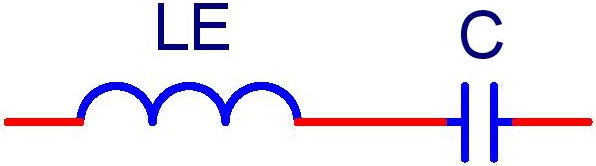
\includegraphics[keepaspectratio=true,width=3in]{./figures/parameters/eslModel.jpg}
\centering
%    \cite{capSite_df_vs_temp}
\caption{ESL Capacitor Model}
\label{eslModel}
\end{figure}


Adding \gls{esl} to the capacitive model creates a new impedance equation (Equation: \eqref{equ:impESL}). Note that for L\textless \textless C, this equation simplifies to Equation: \eqref{equ:capImpEqu} for low frequencies. In other words, the ideal impedance equation can reasonably be used for low frequencies.

\begin{equation}
\label{equ:impESL}
\vec{Z_c} = j\frac{\omega ^2LC - 1}{\omega C}
\end{equation}

\begin{figure}
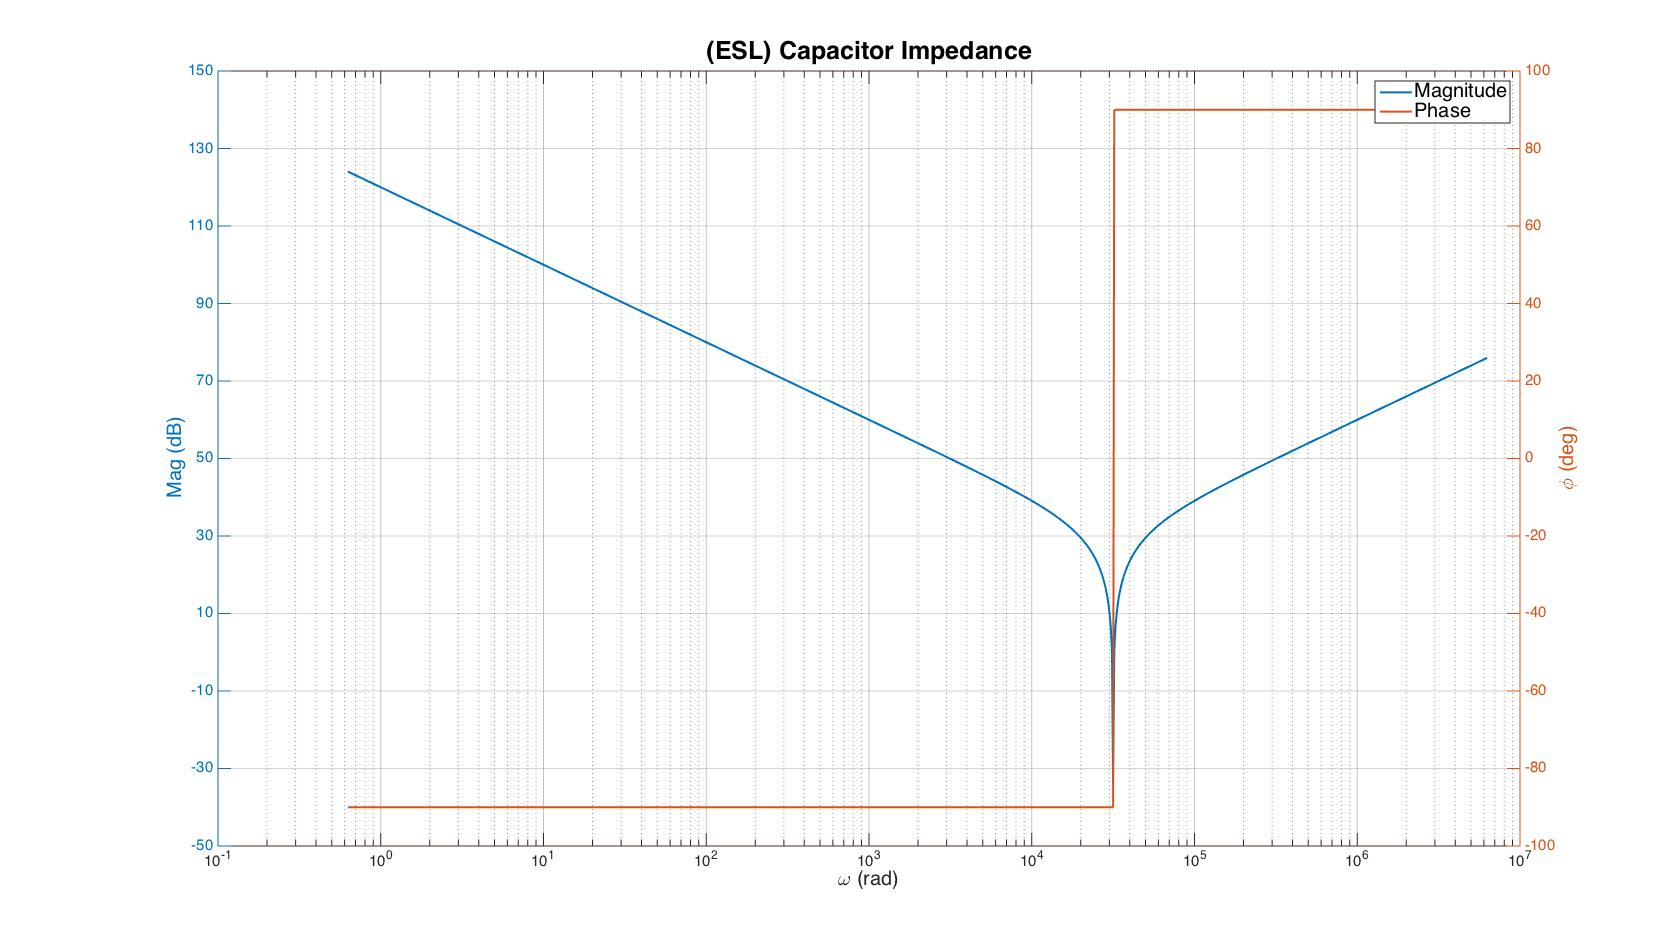
\includegraphics[keepaspectratio=true,width=6in]{./figures/parameters/eslImp.jpg}
\centering
\caption{Capacitor Impedance with ESL}
\label{fig:eslPlot}
\end{figure}


Figure: \ref{fig:eslPlot} shows a graphical representation of a capacitor's magnitude and phase, once \gls{esl} is considered. This plot shows that after the resonance point, the impedance of the inductor (which increases with frequency) begins to dominate. This makes the capacitor ineffective as a bypass element at frequencies higher than its resonance point. Typically, this frequency point and the capacitor's value have an inverse relationship. This is why power supplies and other chips are bypassed by a range of different valued capacitors. 

\subsection{ESR}
\label{sec:ESR}
\begin{figure}
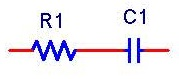
\includegraphics[keepaspectratio=true,width=3in]{./figures/parameters/esrModel.jpg}
\centering
\caption{ESR Capacitor Model}
\label{esrModel}
\end{figure}

The \gls{esr} is the practical result of the fact that the materials used to create a capacitor have resistance. In simple cases, this can be approximated by a resistance in series with the main capacitor (See Figure: \ref{fig:esrModel}).

\gls{esr} becomes important when thinking about DCDC switch mode power supplies. The output ripple voltage of the converter will cause a ripple current to pass through the \gls{esr} and dissipate heat as per Equation: \eqref{equ:dcdcESReqn}. It is important to choose a low \gls{esr} capacitor in order to reduce failures.

\begin{equation}
\label{equ:dcdcESReqn}
P_E = I_{C,RMS}^2 * R_E
~\cite{maxSwEff}
\end{equation}

Another important thing to note about \gls{esr} is that even though it is shown as a resistance in simple models, it is not constant across all frequencies. It is a simplification of the resistive and capacitive elements in a capacitor that are dominated by resistance. That said, it is still sufficient for a basic understanding of a capacitor's impedance (Equation \eqref{equ:ImpCEslEsr}).

\begin{equation}
\label{equ:ImpCEslEsr}
\vec{Z_c} = \frac{1 + j\omega R_EC + (j\omega)^2L_EC}{j\omega C}
\end{equation}

\subsection{Resonance Frequency}
\begin{figure}[ht!]
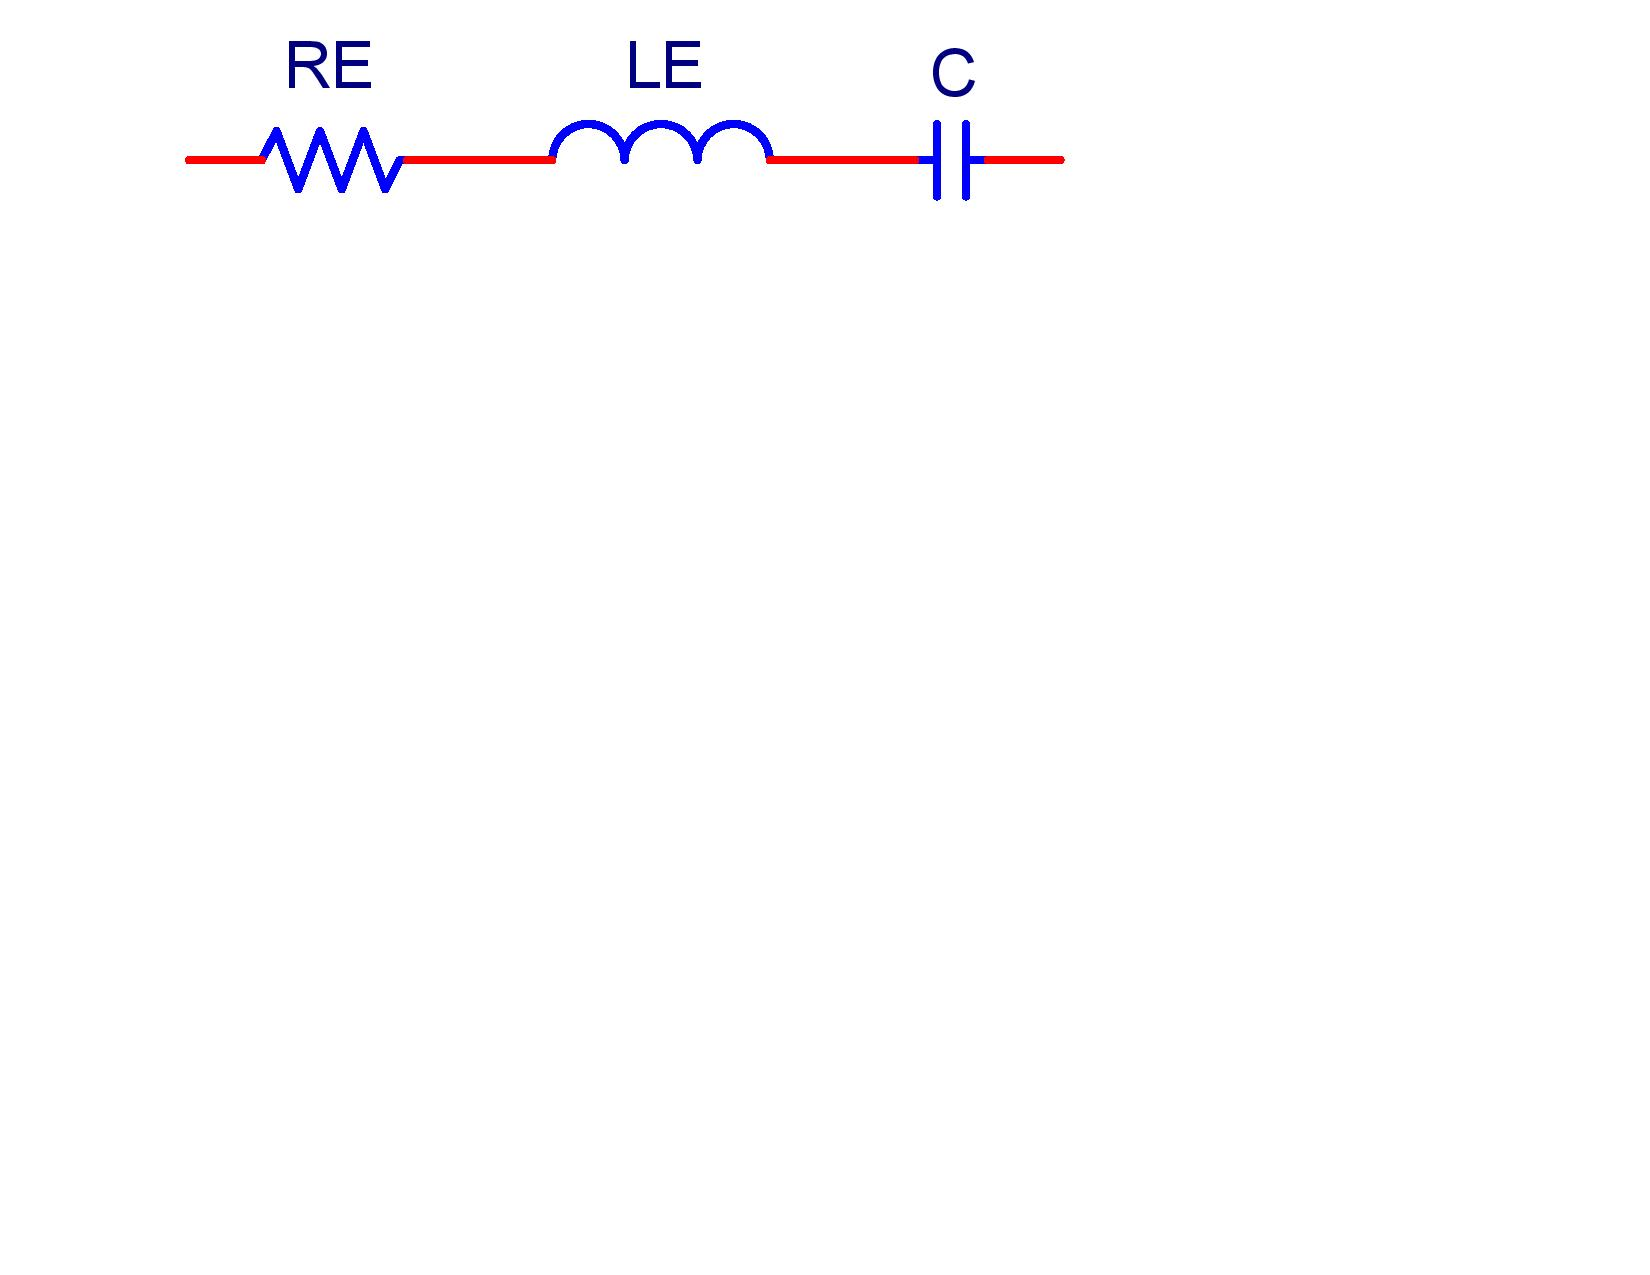
\includegraphics[keepaspectratio=true,width=3in]{./figures/parameters/RLCModel.jpg}
\centering
\caption{RLC Capacitor Model}
\label{fig:RLCModel}
\end{figure}


Once C, \gls{esl}, and \gls{esr} are included into the capacitor model (Figure: \ref{fig:RLCModel}), a parameter known as the self-resonant frequency becomes evident. Equation: \eqref{equ:ImpCEslEsr} shows that when $Z_{ESL} == Z_C$, the capacitor is at its resonance point. At this frequency, the capacitor's impedance is determined solely by the \gls{esr}. This frequency can be calculated by Equation: \eqref{equ:fres}.

\begin{equation}
\label{equ:fres}
f_r = \frac{1}{2\pi \sqrt{LC}}
\end{equation}

\subsection{Dissipation Factor}
\begin{figure}[ht!]
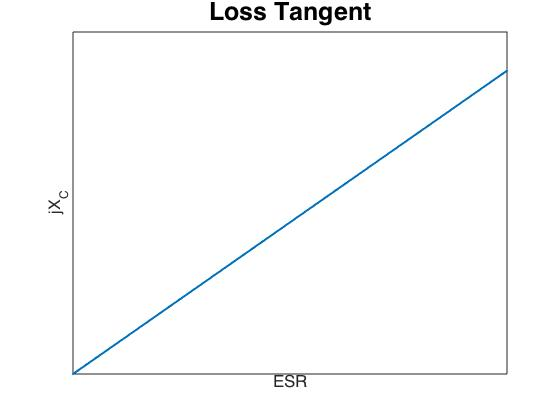
\includegraphics[keepaspectratio=true,width=6in]{./figures/parameters/lossTan.jpg}
\centering
\caption{Loss Tangent}
\label{fig:lossTan}
\end{figure}


The \gls{df}, otherwise known as the loss-tangent, is a measure of the energy stored to the energy dissipated per cycle. It is a measurement of the efficiency of the capacitor. The \gls{df} can be quantified through Equation: \eqref{equ:dispFac}. 

\begin{equation}
\label{equ:dispFac}
D = \frac{R_E}{X_C}
\end{equation}

The loss tangent can be seen in Figure: \ref{fig:lossTan}. The greater the angle, the more efficient the capacitor will be.

\subsection{Quality Factor}

\begin{equation}
\label{equ:qual}
Q = \frac{1}{D}
\end{equation}

The \gls{q} of a capacitor is found by taking the reciprocal of the \acrlong{df}, Equation: \eqref{equ:qual}. It is defined as the ratio of the energy stored to the energy dissipated per cycle.

\subsection{Leakage Resistance}
\begin{figure}[ht!]
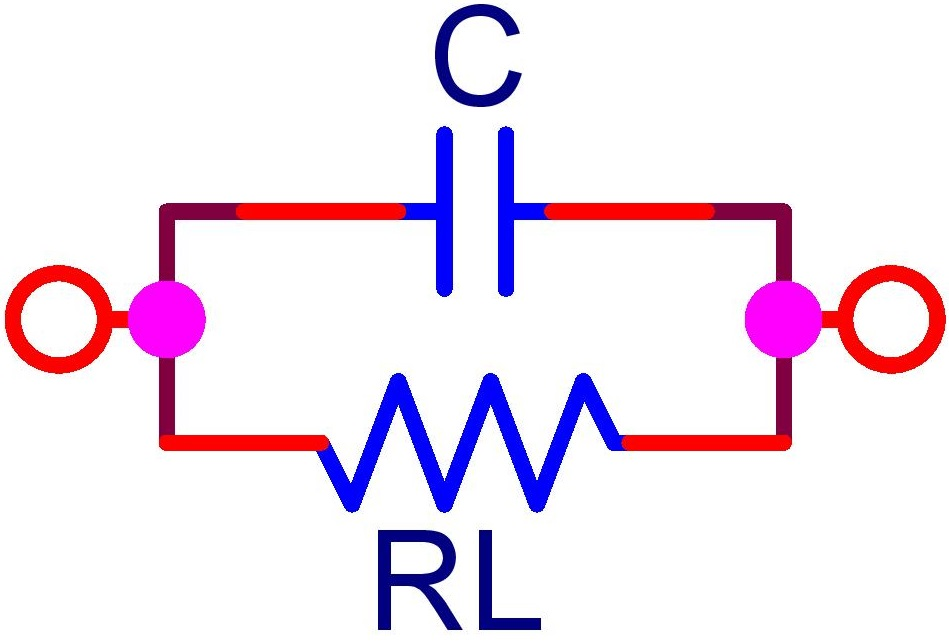
\includegraphics[keepaspectratio=true,width=3in]{./figures/parameters/leakage.jpg}
\centering
\caption{Capacitor Leakage Model}
\label{fig:leakage}
\end{figure}


Every capacitor will have some DC leakage resistance associated with it (Figure:\ref{fig:leakage}). This resistance affects the capacitor's ability to store charge. A capacitor with a high leakage resistance has a low self-discharge rate. This characteristic is especially important in sample and hold circuits.


\subsection{Dielectric Absorption}
\begin{figure}[ht!]
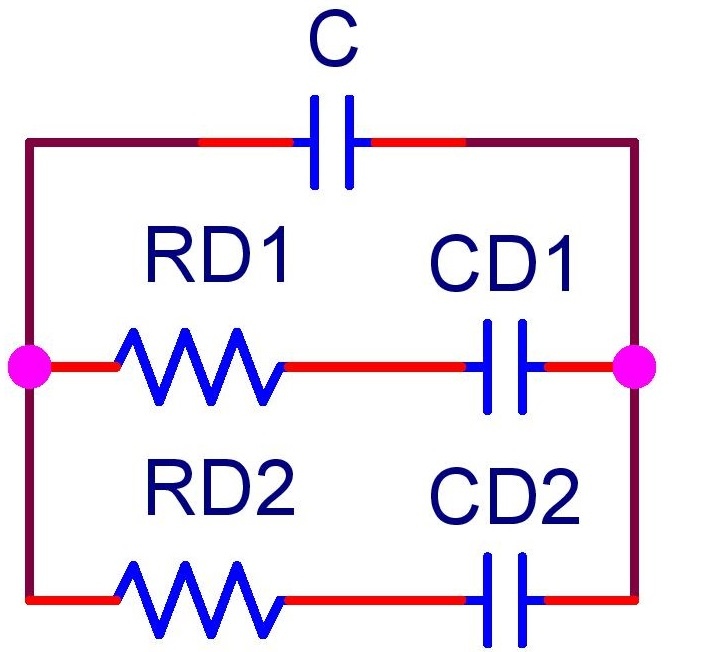
\includegraphics[keepaspectratio=true,scale=.5]{./figures/parameters/dieAbsorption.jpg}
\centering
\caption{Dielectric Absorption}
\label{fig:dieAbsorption}
\end{figure}


\gls{da} in a capacitor is a characteristic which describes the unit's ability to ``regenerate'' a voltage after being shorted to ground for a brief time.

As seen in Figure: \ref{fig:dieAbsorption}, a capacitor can be modeled with multiple RC elements in parallel with the bulk capacitance. When the main capacitor is shorted to ground for a short time and then released, the other capacitors are not guaranteed to have been fully discharged. After several minutes, they can recharge the main capacitance to a significant portion of its original charge. This is why large valued electrolytic capacitors get shipped with a resistor across their terminals.

\subsection{Six Term Model}
\begin{figure}[ht!]
\ifisPPT
\noindent\makebox[\textwidth]{\includegraphics[keepaspectratio=true,width=\paperwidth]{../figures/regression/fullModel.jpg}}
\else
\includegraphics[keepaspectratio=true,width=2in]{./figures/regression/fullModel.jpg}
\fi
\centering
\caption{6 Term Model}
\label{fig:fullModel}
\end{figure}


The model shown in Figure: \ref{fig:fullModel} combines bulk capacitance \gls{esr}, \gls{esl}, leakage, and \gls{da}. It describes a capacitor in simple manner that allows for an understanding of its physical characteristics. It is used in the regression analysis in Section: \ref{sec:regression} to determine the characteristics of unknown capacitors.

\subsection{Murata Model}
\begin{figure}[ht!]
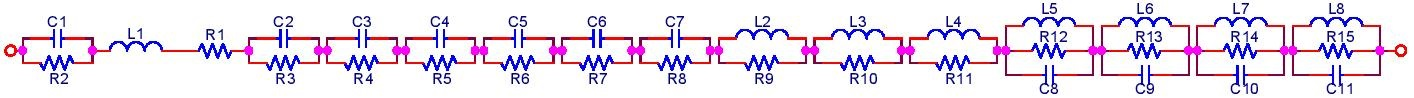
\includegraphics[keepaspectratio=true,width=3in]{./figures/circEx/murataModel.jpg}
\centering
\caption{Murata GRM31MR71H105KA88 Model~\cite{simSurfing}}
\label{fig:murataModel}
\end{figure}



The model shown in Figure: \ref{fig:murataModel} is a functional representation of a ceramic capacitor. It accurately describes how that particular capacitor changes over frequency, but does not lend itself to an intuitive understanding of the physical characteristics of the capacitor. It is used to provide an ideal capacitor frequency response to evaluate the regression analysis in Section: \ref{sec:regression}.

\subsection{Electrochemical Capacitor Model}
\begin{figure}[ht!]
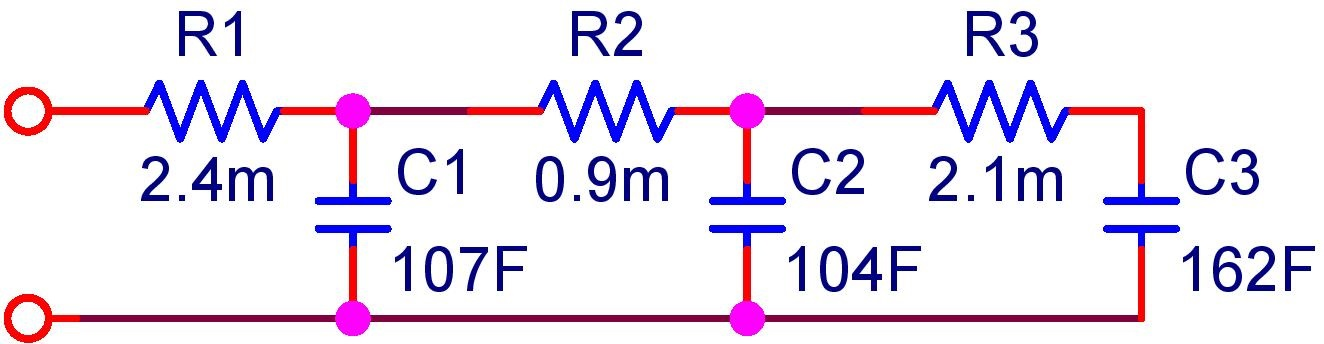
\includegraphics[keepaspectratio=true,width=6in]{./figures/parameters/superCap.jpg}
\centering
\caption{Electrochemical Capacitor \cite{electrochem_intro}[Fig: 8]
\label{fig:superCap}
\end{figure}



The model in Figure: \ref{fig:superCap}, shown by Miller \cite{electrochem_intro}, describes the functionality of an electrochemical capacitor. It has a very high capacitance and several time constants on the order of 10s to 100s of milliseconds. Dependent upon future work, it may be an accurate representation for Titanium based capacitors which have energy and power densities on the same order of magnitude as electrochemical capacitors.

